%\documentclass[twocolumn,oneside,article,9pt]{memoir}
\documentclass[english,a5paper,oneside, onecolumn,article,9pt]{memoir}

\usepackage[english]{babel}
%\usepackage[ansinew]{inputenc}
%\usepackage[T1]{fontenc}
\usepackage{graphicx}
\usepackage{subcaption}
%\usepackage{amsmath,amssymb,amsthm,bm,mathtools}
%\usepackage{lipsum}
%\usepackage{tabularx}
%\usepackage[draft,english,footnote,nomargin]{fixme}
%\usepackage{microtype}
%\usepackage{lmodern}
%\usepackage{hyperref}
%\usepackage{siunitx}
\usepackage[]{algorithm2e}

\usepackage{hyperref}
\hypersetup{
  colorlinks=true,
  linkcolor=red,          % color of internal links
  citecolor=green,        % color of links to bibliography
  filecolor=magenta,      % color of file links
  urlcolor=cyan           % color of external links
}



% Marginer
\setlrmarginsandblock{20mm}{*}{1}
\setulmarginsandblock{20mm}{*}{1.2}
\checkandfixthelayout[nearest]

% Tillad ubalancerede spalter (at de ikke er lige høje)
\raggedbottom

% Indholdsfortengelse
\setsecnumdepth{subsection}
\maxtocdepth{subsection}

%------------- Signature ----------------------
\newcommand\Signature[4]{
  \bigskip
  \begin{@treecolumnfalse}
    \begin{center}
      \begin{tabular}{
          @{\hspace{.05\textwidth}}
          >{\centering\arraybackslash}p{.4\textwidth}
          @{\hspace{.1\textwidth}}
          >{\centering\arraybackslash}p{.4\textwidth}
		  @{\hspace{.05\textwidth}}
          >{\centering\arraybackslash}p{.4\textwidth}
          @{\hspace{.05\textwidth}}}
        \multicolumn{2}{c}{#1, \today} \\[10ex]
        \hrulefill & \hrulefill \\
        #2 & #3 & #4 \\[10ex]
      \end{tabular}
    \end{center}
  \end{@twocolumnfalse}
}
%----------------------------------------------


% Reimplementer \affiliation
%\makeatletter
%\newcommand{\affiliation}[1]{\gdef\@ffiliation{#1}}
%\newcommand{\@ffiliation}{}
%\renewcommand{\maketitlehookc}{\begin{center}\@ffiliation\end{center}}
%\makeatother

%---------------- Basic info ------------------
\title{\Huge{AI4} \Large{ \\ Liquid State Mahine \\ Implementation and Testing}}
\author{Daniel Tang Hviid \\ Dahvi14@student.sdu.dk}
%\setlength\parindent{0pt}

\pagenumbering{gobble}

\begin{document}
%\twocolumn[
\maketitle

\begin{figure}[h]
    \centering
        
\includegraphics[width=0.9\textwidth]{Images/Logo.png}
\end{figure}

\newpage

\begin{centering}
\section*{Abstract}
\end{centering}

Liquid State Machines are a non-differential Neural Network model that contains temporal information with a reservoir hidden layer, that only needs the output layer to be trained.
This paper explains the motive behind implementing a Liquid State Machine, how the theory behind such a model works, goes through the implementation of said model used in this project, and shows qualitative tests of the implementation where individual neurons are investigated.
Finally, this paper shows the Liquid State Machine applied to a sequence prediction problem where the model must correctly predict the next item in the sequence.


\tableofcontents
\newpage

%]
\saythanks

\pagenumbering{arabic}

\chapter{Introduction}

In this paper we go through the motivation behind the project, as well as the theory of the Spiking Neural Network and Reservoir computing, followed by the implementation of a Liquid State Machine in a c++ environment and the tests used to ensure that the implementation works as intended including the prediction of the next item in a repeating sequence.

A Liquid State Machine is a Neural Network model that attempts to more closely resemble a biological brain than other models. It retains temporal information, and is non-differentiable. This makes the model hard to train, which is why this project only looks at training the output layer. It works on the principle that like ripples on a pond contain the information from the stones thrown into the water, spike trains propagating from the initial activation contains information that is unique to that neuron activating.



\section{Motivation}

In this section we look at why Artificial Neural Networks differ from biological neural networks, and why this is worth emulating and investigating. Then we look at some of the ways they can be modified to better emulate the biology of the brain

Standard neural networks are based on mathematical matrix models. These models share little with the functions of the brain, as they are a much oversimplified version of the biological network that constitutes brainmatter.
As biological neural networks have so far unparallelled computational powers and uses, this report is motivated by the idea that these biological networks are worth emulating in search of more powerful and general neural models.

There are several differences between biological neural networks, such as a human brain, and artifical neural networks, such as a feed forward network. These include:

\begin{itemize}
\item Temporal states
\item Non-differential signals
\item Activation functions
\item Structure
\end{itemize}

Looking only at the first three items on this list, there is a artifical neural network model that does take these into considerationg and as such better immitates the workings of the brain. This is the spiking neural network model, which uses the concept of spike trains instead of linear transformations to process the input information. These are said to have higher expressional power than standard neural networks, but in return require more computational power to run.
The last item is structure. A biological brain is not made to be uni-directional, such as a feed-forward neural network, but instead is much better expressed as a reservoir computing framework. When one combines these two extensions of the feed-forward network, one arrives at what is called a Liquid State Machine.

\chapter{Theory}

In this section we look at the teory behind Spiking neural networks, reservoir computing, and Liquid State Machines, assuming that the reader is familiar with Artificial neural networks such as perceptrons, feed-forward networks, and recurrent networks.

\section{Spiking Neural Network}

The main difference between a Spiking Neural Network and a non-Spiking Neural Network is the way it processes the weighted input sum in order to find the output. For a non-Spiking NN, this is the activation function, while a Spiking NN uses a model that stores information from activation to activation. This main difference is what provides the Spiking NN with temporal information that permeates through the network.

Several such models exist, but only the Leaky Integrate-and-fire model \cite{Leaky} will be explained and used in this project. % https://pdfs.semanticscholar.org/8997/95d8e3c07976f62149eb79612e06231d6aee.pdf

The Leaky Integrate-and-fire model attempts to emulate the membrane potential and voltage spikes of a biological neuron. The biological neuron uses two different ion channels in order to build up potential and then dump it as a spike, which is modelled using the following equation, from \cite{leaky}:

\begin{equation}
\tau_m\frac{dv}{dt} = -v(t) + RI(t)
\end{equation}

Where [$\tau_m$] is the time constant, [$v(t)$] is the membrane potential at a given time t, R is the resistance of the membrane, and $I(t)$ is the integral of the input current.
There are three different parts to this. The first is the change in membrane potential; This change in potential is the main part of the equation, as it is what we wish to find at each time step. The second part is the ``leaky'' part of the Leaky Integrate-and-fire, where [$v(t)$] is the membrane potential at a given time t. At each timestep a part of the stored potential is lost, which is proportional in size with the stored potential. The last part is the integral of the weighted inputs, where R is the resistance of the membrane, and $I(t)$ is the integral of the input current, as with a non-Spiking NN. The time constant [$\tau_m$] then scales all of this to fit with the time between each activation.

\section{Reservoir computing}

A reservoir Neural Network is an extension to a recurrent neural network, where the hidden layer is made in such a way that instead of having several layers that feed to each other in order with recurrent connections, the individual neurons are simply randomly connected to each other with random weights.
The input and output layers are then connected to neurons throughout the hidden layer.

\chapter{Implementation}

In this section we look into how the Liquid State Machine was implemented in a code environment, and which choices were made along the way.
The code implementations of this project used C++ as a language, and generally used Object Oriented design philosophy, aiming to be modular and easy to use.

The core of the implementation is the hidden layer of the Liquid State Machine, from now on refered to as the Pool. The Pool have input and output neurons, that are interfaced with by the input and output layers. %(image needed)
The pool is implemented a 3 dimensional tensor of pointers to individual neurons. These neurons each contain a set of parameters, which are outlined in the section below.

\section{Neuron}

The base of the implementation is that of the neuron. This class is responsible for the heavy lifting of the implementation, as it handles the calculations of it's own state, as well as the input and output between individual neurons. Below are subsections explaining the important parameters and structures of class, as well as a class that inherites from the Neuron class.

\subsection{Input and outout}

For every neural network, the neurons must have inputs, $[i]$ and outputs, $[o]$. These inputs are, with the exception of the input layer, the outputs of previous neurons. Often, the input and outputs are stored in matrices, or tensors, as the inputs are calculated by applying the input weights to the outputs. In this implementation, however, whenever a neuron activates it calls every neuron that it is connected to and adds the corrossponding weight to the collected input of that neuron. This is done because in a spiking neural network the output is either one or zero, and at any given activation step it is to be expected that the majority of neurons are not activating, thus saving computations. It should be noted that these savings could also be achieved through a sparse matrix or tensor, and tha tlibraries exist that do these kinds of calculations very efficiently, but this method was chosen for simplicity of implementation.

\subsection{Membrane potential}

Normally, the input is reset for after each activation of the neural network; However, when using spiking neurons the input spills over to the next activation. This spillover is called the membrane potential \cite{leaky}, $[u]$. This internal value is what determines whether or not the neuron spikes to produce an output. Because a leaky-integrate-and-fire \ref{leaky_model} model is used  this value will decrease over time if it is not increased by other neurons spiking.

\subsection{Synapses}

Because this implementation does not include a matrix multiplication method, the inputs of each neuron is calculated through the use of synapses; Each neuron contains a list of pointers to other neurons as well as a list of weights. Each pointer-weight pair is called a synapse, as they mirror the synaptic nature of a biological neural network. When a neuron activates it will call a method of the neuron corrosponding to each of the pointers that increases it's input by the amount equal to the weight of the synapse.

\subsection{Output neuron}

In a Liquid State Machine the output layer is a bit special. Because of the nature of the spiking models, it can be ver hard to train spiking neurons, and as such we want to do it as sparsely as possible. Because of this, having the output layer be the only part that is trained is an enticing option. This, however, is hard to achieve if the synapses are used for output, as it is in the standard Neuron class of this implementation. Because of this, the output neurons pull outputs from it's inputs, as opposed to pushing it's output to other neurons.

\section{Algorithm}

Now that the elements are accounted for, the algorithm that is run each time the LSM is activated can be explained. As can be seen in \ref{Alg:activation}, each tme the network is activated it goes through four steps: \textbf{Inputs}, \textbf{Check Activity}, \textbf{Activate Neurons}, and \textbf{Output Neurons}. \textbf{Inputs} translates the network input into inputs for the input layer, and checks if they should be added to the list of active neurons. Then \textbf{Check Activity} adds all active neurons to the list of active neurons, before \textbf{Activate Neurons} activates all neurons with a high enough membrane potential. Finally, \textbf{Output Neurons} activates it's synapses and checks if it spikes. The output neurons needs to do this in reverse order because they pull the activations, instead of pushing them.

\begin{algorithm}
\caption{The main algorithm of the LSM implementation. Input and Output layers are partly seperated from the pool for simplicity and modularity.}
\label{Alg:activation}
\KwData{Input values}
\KwResult{Output values}
	Step 1 : Inputs\;
	\ForAll{Input Neurons}{
		Apply provided input value\;
		\If{$Membrane Potential \geq Spiking Potential$}{
			Add neuron to Active Neurons List\;
		}
	}
	Step 2 : Check Activity\;
	\ForAll{Pool Neurons}{
		\If{$Membrane Potential \geq Spiking Potential$}{
			Add neuron to Active Neurons List\;
		}
	}
	Step 3 : Activate Neurons\;
	\ForAll{Neurons in Active Neurons List}{
		Activate all synapses\;
	}
	Step 4 : Output Neurons\;
	\ForAll{Output Neurons}{
		Activate all synapses\;
		\If{$Membrane Potential \geq Spiking Potential$}{
		Set output to 1\;
		}
	}
	Output active Neurons\;
\end{algorithm}

Finally, this leaves a set of output values corresponding to which of the output neurons have been activated. This, however, does not necessarily translate very well into a readable output, as output neurons cannot be expected to spike every activation.

One way of translating the output is to look at the membrane potential of the output layer instead of the spikes. This provides information about how close the neuron is to outputting, which is useful for training, but has the disadvantage of being low right after a spike has occured.
Another approach is to average the spikes of several sequential activations, thereby looking at the frequency of the spikes. This can also be used for training, but contains less information if only a single, or few, spikes occur.

Finally, one can use both. By looking at both the internal value as well as the spikes, and averaging this value over several activations, enough information is stored about the frequency of the spikes, as well as the lead-up to each spike.



\chapter{Testing}

This section documents the tests used to ensure that the implementation of Liquid State Machine is functional, and to highlight certain properties of both the implementation and the network model itself.

\section{Neuron model}

There exists several neural models that can be used for a Liquid State Machine, or a Spiking Neural Network. The selected model is the Leaky-Integrate-and-Fire model \ref{sec:leaky}, as it is simple, not computationally heavy, and expressive enough for this project.

In order to test this model, a baseline set of parameters must first be selected. The baseline parameters can be found in table \ref{tab:neuron}. For these parameters, the model behaves as can be seen in figure \ref{fig:model1} which is clearly a smooth membrane potential curve followed by a spike as the potential reaches the spiking threshold. In figure \ref{fig:model2}, the parameters have been changed to allow a random input between zero and one, thus illustrating how a neuron would act when it's input is affected by several synapses that fire independent of each other. It is clear from these two images, as the neuron fires in exactly the same timestep, that the mean input is relevant, even if the input is not consistent.

\begin{table}[h]
\centering
\begin{tabular}{cccc}
Resistance & Time constant & Resting potential & Spiking potential\\
2.2 & 10 & 0 & 1  
\end{tabular}
\caption{Table of parameters used when testing neuron activity.}
\label{tab:neuron}
\end{table}

\begin{figure}
    \centering
    \begin{subfigure}[b]{0.3\textwidth}
        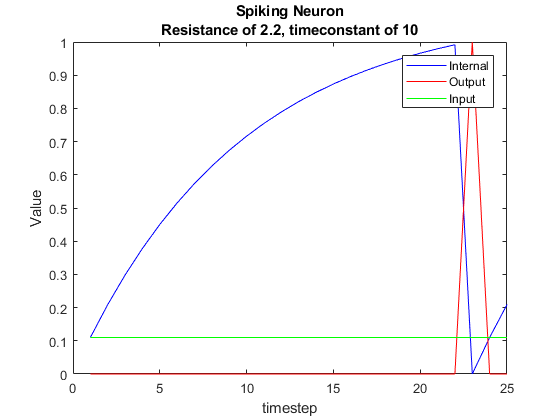
\includegraphics[width=\textwidth]{Images/slow.png}
        \caption{The neuron model using the baseline parameters and constant input of 0.5.}
        \label{fig:implementation_test}
    \end{subfigure}
    \begin{subfigure}[b]{0.3\textwidth}
        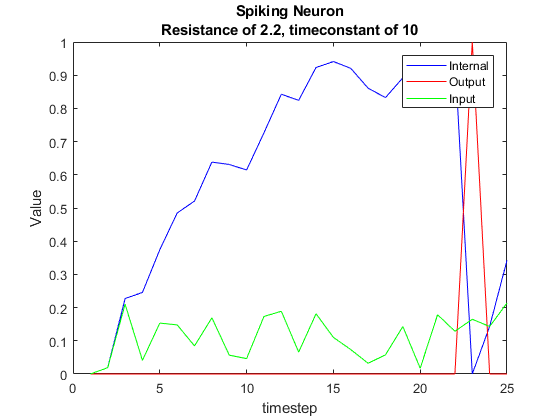
\includegraphics[width=\textwidth]{Images/randomInput.png}
        \caption{The neuron model using the baseline parameters and random input with a mean of 0.5.}
        \label{fig:implementation_test}
    \end{subfigure}
    \begin{subfigure}[b]{0.3\textwidth}
        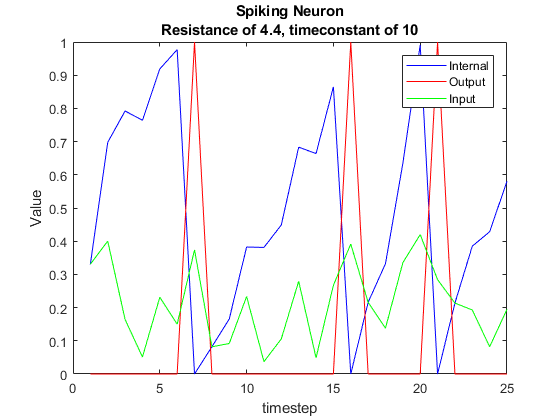
\includegraphics[width=\textwidth]{Images/fast.png}
        \caption{The neuron model using double resistance, and random input with a mean of 0.5.}
        \label{fig:implementation_test}
    \end{subfigure}
    \caption{Tests of the neuron model.(a) shows the ideal potential curve followed by a spike. (b) shows how the potential curve caused by a randomized input can be used in place of the ideal curve to get the same frequency of the spike. (c) shows how doubling the resistance parameter does not double the fireing rate of the neuron.}
    \label{fig:implementation_test}
\end{figure}

If one instead changes the parameters so that the resistance is twice of what it was in the baseline, and sets the input to a random number between zero and one each timestep, the result, as seen in figure \ref{fig:fast}, the neuron fires three times in the same timestep, showing how the resistance is not proportional to the fire rate of the neuron.

\section{Propagation}

In a functional Liquid State Machine, the activation of a neuron in the hidden layer will spread to nearby neurons like ripples in a pond. In order to test this, one can activate a single neuron and observe this behavior through the activation of the connected neurons. One way of performing this observation is by setting the neuron parameters in such a way that a single received pulse is enough to cause an activation, and then activating a single neuron in the reservoir. The expected behavior is a cascade effect where each activation will activate several other neurons, eventually activating each connected neuron in the reservoir.

By visualizing the activity of the network through repeated activations, this is easy to test. In figure \ref{fig:implementation_test}, it is clear that a single reservoir neuron is activated after the first timestep, and that after ten timesteps all connected neurons have been activated. In this figure it is also clear that three adjacent neurons, which is the number of connections each neuron have, are activated in the second timestep, as is expected from a functional Liquid State Machine.

\begin{figure}
    \centering
    \begin{subfigure}[b]{0.225\textwidth}
        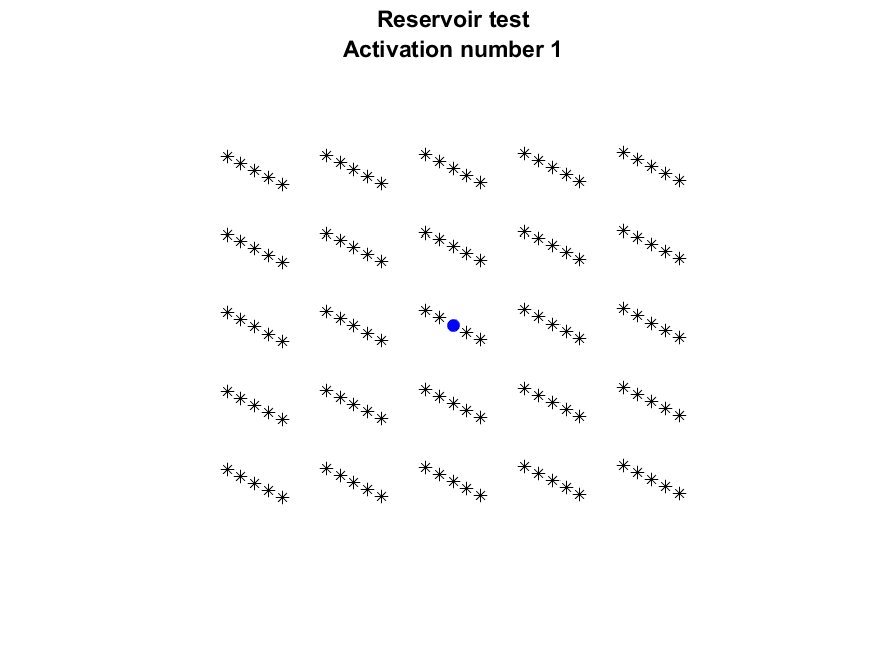
\includegraphics[width=\textwidth]{Images/Reservoir_test_Activation_number_1.png}
        \caption{The test network after a single timestep.}
    \end{subfigure}
    \begin{subfigure}[b]{0.225\textwidth}
        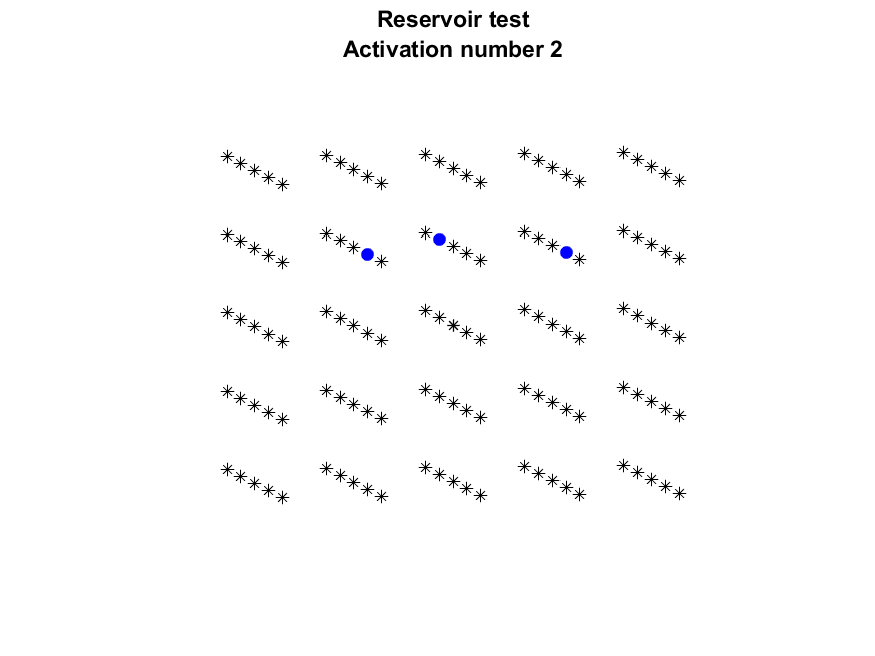
\includegraphics[width=\textwidth]{Images/Reservoir_test_Activation_number_2.png}
        \caption{The test network after two timesteps.}
    \end{subfigure}
    \begin{subfigure}[b]{0.225\textwidth}
        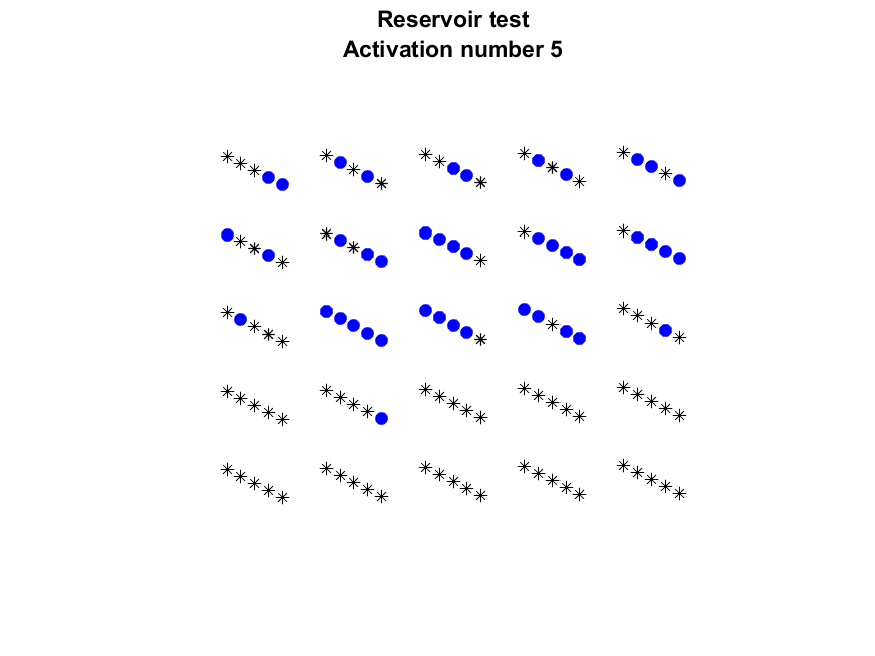
\includegraphics[width=\textwidth]{Images/Reservoir_test_Activation_number_5.png}
        \caption{The test network after five timesteps.}
    \end{subfigure}
     \begin{subfigure}[b]{0.225\textwidth}
        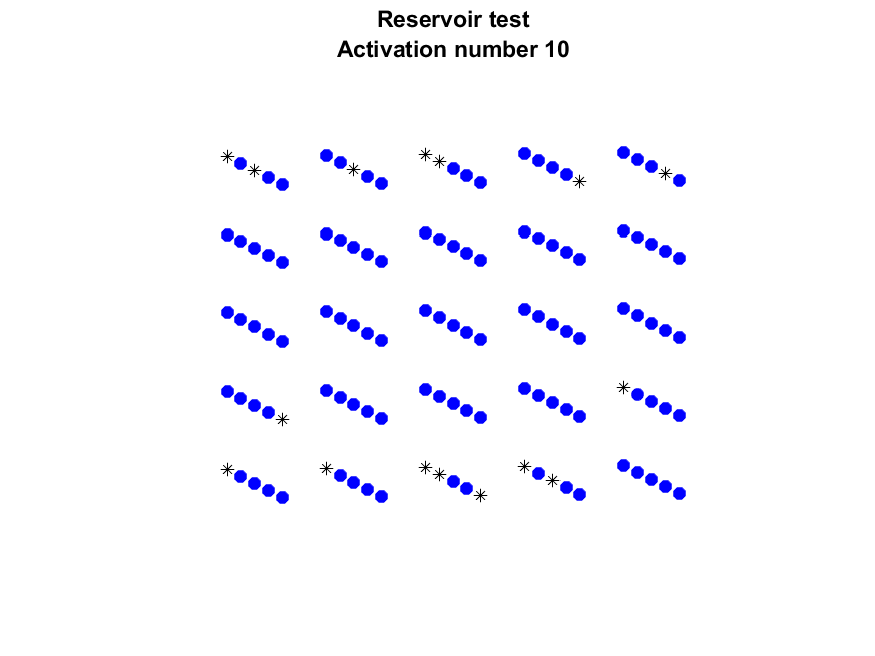
\includegraphics[width=\textwidth]{Images/Reservoir_test_Activation_number_10.png}
        \caption{The test network after ten timesteps.}
    \end{subfigure}
    \caption{Test of the propagation of the network. Every neuron has three synapses which are adjacent to it, and each spike will activate all three synases. After the first timestep, only the selected neuron is active. In the second timetep, it has spiked and is therefore inactive while the three neurons it has synapses to are active. After five timesteps a large proportion of the neurons are active, and after ten all connected neurons are active.}
    \label{fig:implementation_test}
\end{figure}

\section{Reservoir activity}

The reservoir parameters are as important as the neuron parameters. There are several parameters that can be tuned and modified, and in this section the number of connections as well as the proportion of exitory to inhibitory neurons are tuned. The rest of the parameters are kept constant, as well as the neuron parameters, which can be found in table \ref{tab:reservoir}.

\begin{table}[h]
\centering
\begin{tabular}{cccc}
Resistance & Time constant & Resting potential & Spiking potential\\
2.2 & 10 & 0 & 1
\end{tabular}
\begin{tabular}{ccc}
Min weight & Max weight & Max synapse length\\
0 & 1 & 2
\end{tabular}
\begin{tabular}{cc}
Input neurons & Connections per input neuron\\
3 & 10
\end{tabular}
\caption{Table of parameters used for testing network activity when testing different amounts of connectors per neuron.}
\label{tab:reservoir}
\end{table}

 Having too few connections will result in low amount of activity that won't spread beyond the input neurons. Conversely, having too many connections will result in a cascade of activity that results in all, or most, neurons activating every timestep. Both of these options are equally useless, as they provide essentially constant output.

First, to test the impact of the number of connections that each neuron have on the level of activity of the reservoir, two different amounts of neuron connections are tested. The reservoir after one hundred timestept with six and seven connections per neuron can be seen in figure \ref{fig:reservoir_6} and \ref{fig:reservoir_7}. As can be seen in the first image, six connections are enough to provide a good level of activity throughout the network, without having a lot of the neurons activate each timestep. On the other hand, having seven connections is enough to cause a run-away reaction that activates almost all the neurons each timestep. Clearly, there is a fine balance between having enough connections, and having too many.

A way of correcting this is by including inhibitory neurons. In figure \ref{fig:reservoir_7_in} we see how 15\% inhibitory neurons brought the level of activity back down, and in figure \ref{fig:reservoir_10_in}.

\begin{figure}
    \centering
    \begin{subfigure}[b]{0.4\textwidth}
        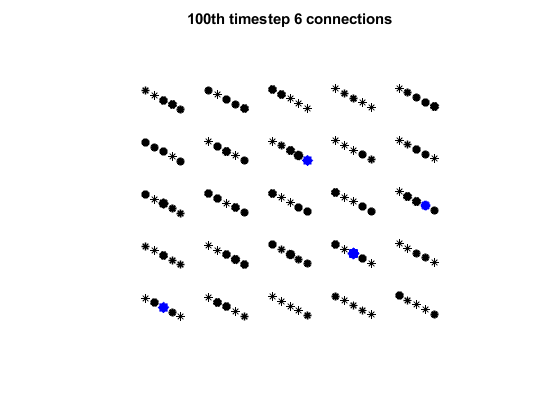
\includegraphics[width=\textwidth]{Images/pool_6_100.png}
        \caption{The test network after a hundred timesteps with 6 connections per neuron.}
    \label{fig:reservoir_6}
    \end{subfigure}
    \begin{subfigure}[b]{0.4\textwidth}
        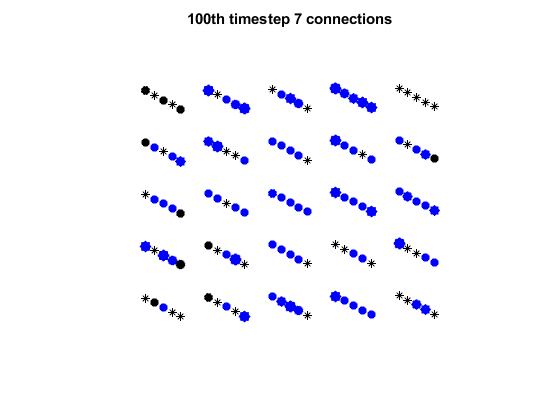
\includegraphics[width=\textwidth]{Images/pool_7_100.png}
        \caption{The test network after a hundred timesteps with 7 connections per neuron.}
    \label{fig:reservoir_7}
    \end{subfigure}
    \begin{subfigure}[b]{0.4\textwidth}
        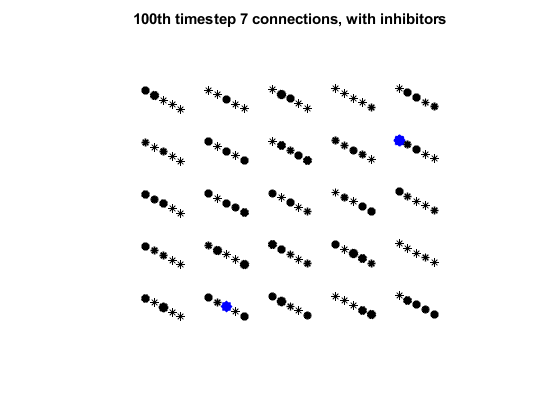
\includegraphics[width=\textwidth]{Images/pool_7_100_s.png}
        \caption{The test network after a hundred timesteps with 7 connections per neuron, with inhibitors.}
    \label{fig:reservoir_7_in}
    \end{subfigure}
     \begin{subfigure}[b]{0.4\textwidth}
        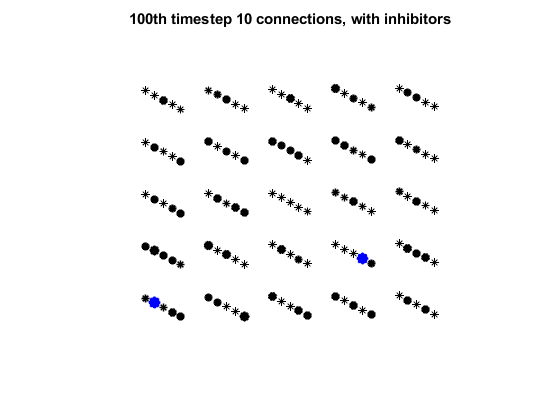
\includegraphics[width=\textwidth]{Images/pool_10_100_s.png}
        \caption{The test network after a hundred timesteps with 10 connections per neuron, with inhibitors.}
    \label{fig:reservoir_10_in}
    \end{subfigure}
    \caption{Spikes and membrane potential after a hundred timesteps with different amounts of connections per neuron and inhibitors.}
\end{figure}

\section{Training}
















\section{Discussion}

In this section we discuss the Liquid State Machine, more specifically the choises taken when implementing it, the troubles of tuning it, and the results of the tests.

When implementing a neural network, one would usually make a set of matrices and tensors that contain the inputs, outputs, activations and weights. In this implementation, however, a graph implementation with nodes for neurons was used. This impacted the computational time of the network, but also allowed for easier bugfixing and faster implementation. This tradeoff was made because of the limited scope of the project, as well as the relatively small problem it was used on. This allowed for the implementation of the Neuron class, which made it much easier to implement it in a modular fashion.

Tuning a Liquid State Machine is a tedious process, as a small change in parameters will make the network lose a lot of accuracy. In particular the number of connections, neuron resistance, resting potential, proportion of inhibatory neurons, and number of synapses per input neurons. These parameters should be tuned quite gently, as they will make the network either almost inactive or start a chain reaction.

\section{Conclusion}

\begin{thebibliography}{9}

\bibitem{leaky}
 Hélène Paugam-Moisy and Sander Bohte\\
 Computing with Spiking Neuron Networks\\
 \textit{pdfs.semanticscholar.org/8997/95d8e3c07976f62149eb79612e06231d6aee.pdf}

\end{thebibliography}





\end{document}

